\section{The optimal order-averaged Euler constant}
\label{ord:sec:main}
The incoming report \cite[Sections 2 and 9]{IncomingBounds} proves
that the optimal order-uniform scaled remainder tends to one and gives
a matching candidate lower asymptotic. Its upper asymptotic remains an
explicit conjecture there. We prove that conjecture, identify the eventual
maximizing boundary, and determine a further asymptotic scale.

Write
\[
 \begin{gathered}
 d_j(a,b)=\sum_{n=0}^j(-1)^n\binom jn
              \frac{H_{2n}^{(b)}}{(2n+1)^a},\qquad
 E_N(a,b)=\sum_{j=0}^{N-1}\frac{d_j(a,b)}{2^{j+1}},\\
 R_N(a,b)=2^N(E_N(a,b)-g_{a,b}).
 \end{gathered}
\]
Let $T_a,U_b$ be independent gamma variables of rate one and shapes
$a,b$, with $T_0=0$. To avoid confusing the logarithmic kernel with the
polylogarithm $F_{a,b}$, put
\begin{equation}\label{ord:eq:psi-J}
 \Psi_N(t)=f_N(e^{-2t}),\qquad J_N(s)=\E\Psi_N(T_s),\qquad J_N(0)=0.
\end{equation}
The existing positive two-measure identity is
\begin{equation}\label{ord:eq:remainder}
 R_N(a,b)=\E\frac{\Psi_N(T_a+U_b)-\Psi_N(T_a)}{1-e^{-U_b}}.
\end{equation}
It holds for $a\ge0,b>0$; in particular it does not require a finite
unweighted signed moment measure. Expanding the denominator into a
positive geometric series and using gamma addition gives, for $b>1$,
\begin{equation}\label{ord:eq:first-gamma}
 0\le R_N(a,b)-\{J_N(a+b)-J_N(a)\}\le\zeta(b)-1.
\end{equation}
For completeness, multiplication of the density of $U_b$ by
$e^{-(r-1)U_b}$ gives $r^{-b}$ times a gamma density of rate $r$.
The term $r=1$ is the displayed difference of $J_N$ values, while each
remaining expectation is between zero and one. Tonelli's theorem
justifies the sum.

We also use the previously proved bound
\begin{equation}\label{ord:eq:inherited-one}
 0<R_N(a,b)<1\qquad(a\ge1,b>0),
\end{equation}
from the manuscript's extended one-sided Euler theorem
\cite[Chapter 5, \texttt{05-real-euler.tex}]{ProveIt}. We identify this
input explicitly: the universal constant greater than one alone would
not replace it in the proof below.

\subsection{Eventual reduction to the outer-order axis}

Define
\begin{equation}\label{ord:eq:axis}
 A_N(b)=R_N(0,b)
 =\frac1{\Gamma(b)}\int_0^\infty t^{b-1}e^{-t}
       k_N(e^{-t})\dd t,
 \qquad
 k_N(v)=\frac{(1+v)(1-v^2)^{N-1}}{1+v^2}.
\end{equation}
All limits of truncation indices in this section are through positive
integers.

\begin{theorem}[Eventual exact axis reduction]\label{ord:thm:axis-reduction}
For all sufficiently large $N$,
\begin{equation}\label{ord:eq:axis-reduction}
 C_N:=\sup_{a,b>0}R_N(a,b)=\max_{b>0}A_N(b)>1.
\end{equation}
The supremum over positive orders is not attained. If $a=0$ is admitted,
every global maximizer is on that axis. Moreover, $C_{N+1}<C_N$ for
all sufficiently large $N$.
\end{theorem}

\begin{proof}
Put $L=\log N$. We separate $b\ge3L/2$ from $b\le3L/2$, always
assuming $N$ large enough for the indicated intervals to be nonempty.

\emph{Comparison above the cutoff.}
The function $f_N$ is decreasing and convex on $[0,1]$, and
$0\le-f_N'(x)\le N+1$. Thus, for $0\le r,v\le1$,
\[
 f_N(rv^2)-f_N(v^2)\le(N+1)(1-r)v^2.
\]
Subtract the axis integrand from \eqref{ord:eq:remainder} and set
$r=e^{-2T_a}$, $v=e^{-U_b}$. Independence gives the useful uniform
comparison
\begin{equation}\label{ord:eq:axis-comparison}
 \begin{split}
 R_N(a,b)-A_N(b)\le{}&
 (N+1)(1-3^{-a})\{\zeta(b)-1-2^{-b}\}\\
 &-J_N(a)\zeta(b),\qquad b>1.
 \end{split}
\end{equation}
Indeed $\E(1-r)=1-3^{-a}$,
$\E[v^2/(1-v)]=\zeta(b)-1-2^{-b}$, and
$\E[1/(1-v)]=\zeta(b)$.

For $0<a\le1$ there is an elementary lower bound
\begin{equation}\label{ord:eq:J-lower}
 J_N(a)\ge\frac{ae^{-2}}{L+4}N^{-1/2}.
\end{equation}
To prove it, restrict the defining integral to
$t\in[L/2+1,L/2+2]$. Bernoulli's inequality gives
\[
 \Psi_N(t)\ge1-(N+1)e^{-2t}\ge1-2e^{-2}>\frac12.
\]
Log convexity of the gamma function gives $\Gamma(a+1)\le1$ for
$0\le a\le1$, and hence $1/\Gamma(a)\ge a$. Also
$t^{a-1}\ge1/t$ on the interval in question, and
$e^{-t}\ge e^{-2}N^{-1/2}$. Its length is one, proving
\eqref{ord:eq:J-lower}.

For $b\ge2$, integral comparison gives
\[
 \zeta(b)-1-2^{-b}
 \le3^{-b}\left(1+\frac3{b-1}\right)\le4\,3^{-b}.
\]
Consequently the positive term in \eqref{ord:eq:axis-comparison}, for
$0<a\le1$ and $b\ge3L/2$, is at most
\[
 8a\log3\,N^{1-(3/2)\log3}.
\]
Its ratio to the right side of \eqref{ord:eq:J-lower} is bounded by
\[
 8e^2\log3\,(L+4)
       e^{-(3/2)(\log3-1)L}\longrightarrow0.
\]
We have therefore proved, uniformly on this parameter region,
\begin{equation}\label{ord:eq:strict-axis-gap}
 R_N(a,b)\le A_N(b)-\frac{ae^{-2}}{2(L+4)}N^{-1/2}
 \qquad(0<a\le1,\ b\ge3L/2)
\end{equation}
for all sufficiently large $N$.

\emph{Exclusion below the cutoff.}
Monotonicity of $J_N$ in its gamma shape and
\eqref{ord:eq:first-gamma} give
\begin{equation}\label{ord:eq:small-b-upper}
 R_N(a,b)\le J_N(b+1)+\zeta(b)-1
       \qquad(0\le a\le1,\ b>1).
\end{equation}
Since $\Psi_N(L/2)=f_N(1/N)\le e^{-1}$,
\begin{equation}\label{ord:eq:deficit-cdf}
 1-J_N(s)\ge(1-e^{-1})
          \Pr\{T_s\le L/2\}.
\end{equation}
For every fixed $D>1/2$ there is $c_D>0$ such that
\begin{equation}\label{ord:eq:gamma-lower-tail}
 \Pr\{T_{DL+1}\le L/2\}
 \ge c_D L^{-1/2}e^{-I(D)L},\qquad
 I(D)=\frac12-D+D\log(2D),
\end{equation}
for all sufficiently large $L$. This lower bound follows directly by
integrating the gamma density over $[L/2-1,L/2]$:
\[
 \Pr\{T_{DL+1}\le L/2\}
 \ge\frac{(L/2-1)^{DL}e^{-L/2}}{\Gamma(DL+1)}.
\]
Stirling's formula \cite[Section 5.11]{DLMF} supplies
\eqref{ord:eq:gamma-lower-tail}; no
large-deviation equivalence is needed.

On $4\le b\le L/2$, gamma stochastic ordering and the central limit
theorem imply that the lower bound in \eqref{ord:eq:deficit-cdf}
eventually exceeds $1/5$ uniformly, since at the worst endpoint
$\Pr\{T_{L/2+1}\le L/2\}\to1/2$. The central limit theorem here follows
from
\[
 \E e^{it(T_s-s)/\sqrt s}
 =e^{-it\sqrt s}(1-it/\sqrt s)^{-s}\longrightarrow e^{-t^2/2}.
\]
On the other hand $\zeta(b)-1\le\zeta(4)-1\le5/48<1/5$.
On $L/2\le b\le L$, apply \eqref{ord:eq:gamma-lower-tail} with $D=1$.
The deficit is bounded below by a positive constant times
\[
 L^{-1/2}N^{-(\log2-1/2)},
\]
whereas $\zeta(b)-1\le2N^{-(\log2)/2}$. The former dominates because
$\log2-1/2<(\log2)/2$.
On $L\le b\le3L/2$, take $D=3/2$. The corresponding deficit is at least
a positive constant times
\[
 L^{-1/2}N^{-((3/2)\log3-1)},
\]
whereas $\zeta(b)-1\le2N^{-\log2}$. Again the deficit dominates:
$(3/2)\log3-1<\log2$. The last inequality is equivalent to
$3\sqrt3<2e$; for example $e>8/3$ and $3\sqrt3<16/3$ prove it.
Thus \eqref{ord:eq:small-b-upper} is strictly below one throughout
$4\le b\le3L/2$ for large $N$.

The bounded rectangle $0\le a\le1$, $0<b\le4$ is also uniform.
Couple $T_a\le T_1$ and $U_b\le U_4$. The derivative satisfies
$0\le\Psi_N'\le4$, and its supremum on every bounded interval tends
to zero. Indeed, with $v=e^{-2t}$, its two positive terms are bounded
by $2Nv(1-v)^{N-1}\le2$ and $2v/(1+v)^2\le1/2$.
The actual terms contain $(1-v)^{N-1}$ and $(1-v)^N$, respectively,
which give uniform decay on every fixed bounded $t$-interval.
Since $u/(1-e^{-u})\le1+u$, we obtain
\[
 R_N(a,b)\le\E\left[(1+U_4)
          \sup_{0\le t\le T_1+U_4}\Psi_N'(t)\right].
\]
The integrand tends to zero and is bounded by $4(1+U_4)$.
Dominated convergence therefore proves uniform convergence to zero on
the bounded rectangle and completes the exclusion below $3L/2$.

Finally, \eqref{ord:eq:inherited-one} excludes $a\ge1$. The function
$A_N$ is continuous, tends to zero as $b\downarrow0$ for $N\ge2$, and
tends to one as $b\to\infty$. The elementary expansion established
below shows that $A_N(b)>1$ for all sufficiently large $b$ at each fixed
$N$. Its maximum is therefore attained and exceeds one. Every positive
outer order is strictly inferior either to one or to its corresponding
axis value, while continuity as $a\downarrow0$ approaches each axis
value. Finally, $A_{N+1}(b)<A_N(b)$ at every $b>0$ by its positive
integral. If $b'$ maximizes $A_{N+1}$ and both indices are in the proved
range, then
\[
 C_{N+1}=A_{N+1}(b')<A_N(b')\le C_N.
\]
This proves eventual strict monotonicity as well.
\end{proof}

\subsection{Resolution of the asymptotic-constant conjecture}

Set
\begin{equation}\label{ord:eq:constants}
 \begin{gathered}
 h=\log(3/2),\qquad \alpha=h^{-1},\qquad
 p=\frac{\log2}{h},\qquad q=\frac{\log3}{\log2},\\
 d_0=\alpha\log q,\qquad
 \widehat b_N=\alpha\log N+d_0=\frac{\log(Nq)}h,\qquad
 c=(1-q^{-1})q^{-p}.
 \end{gathered}
\end{equation}

\begin{lemma}[Axis sign changes and a Taylor enclosure]\label{ord:lem:axis}
For $N\ge2$, $k_N(v)-1$ has exactly one zero in $(0,1)$, with positive
sign before it and negative sign after it. Consequently, if
$A_N(b_0)<1$, then $A_N(b)<1$ for $0<b<b_0$.
For every $N\ge1$ and $b>0$,
\begin{equation}\label{ord:eq:axis-taylor}
 \begin{split}
 A_N(b)&=1+2^{-b}-N3^{-b}-N4^{-b}+\eps_N(b),\\
 0&\le\eps_N(b)\le\frac{N^2-N+2}{2}(5^{-b}+6^{-b}).
 \end{split}
\end{equation}
\end{lemma}
\begin{proof}
The numerator determining the sign of the logarithmic derivative of
$k_N$ on $(0,1)$ is
\[
 P_N(v)=1-(2N+1)v+v^2+(3-2N)v^3.
\]
For $N\ge2$, its derivative is strictly negative on $[0,1]$.
Since $P_N(0)>0>P_N(1)$, the function $k_N$ first increases and then
decreases. Its endpoint values are one and zero, proving the claimed
single crossing.
In the variable $t=-\log v$, the signed function $k_N(e^{-t})-1$ is
negative before a unique $t_0>0$ and positive after it. If $b<b_0$,
multiplication by $t^{b-b_0}$ changes its integral by at most multiplication
by $t_0^{b-b_0}$: the factor is larger on the negative part and smaller
on the positive part. This proves the implication for $A_N$ after
normalizing by the positive gamma factors.

For the enclosure put $G_N(x)=(1-x)^{N-1}/(1+x)$. Its second derivative
is nonnegative and bounded by $N^2-N+2$ on $[0,1]$. For $N\ge3$,
\[
 G_N''(x)=
 \frac{(N-1)(N-2)(1-x)^{N-3}}{1+x}
 +\frac{2(N-1)(1-x)^{N-2}}{(1+x)^2}
 +\frac{2(1-x)^{N-1}}{(1+x)^3};
\]
$N=1,2$ are checked directly. Since $G_N(0)=1$ and $G_N'(0)=-N$,
Taylor's integral remainder gives
\[
 0\le G_N(x)-1+Nx\le\frac{N^2-N+2}{2}x^2.
\]
Multiply by $1+v$, substitute $x=v^2$, and use
$\E e^{-jU_b}=(j+1)^{-b}$.
\end{proof}

\begin{theorem}[Sharp late Euler constant and unique axis maximizer]
\label{ord:thm:leading}
The conjecture of \cite[Section 9]{IncomingBounds} holds:
\begin{equation}\label{ord:eq:sharp-asymptotic}
 C_N-1\sim cN^{-p}.
\end{equation}
For all sufficiently large $N$, $A_N$ has a unique global maximizer
$b_N$, and
\begin{equation}\label{ord:eq:axis-location}
 b_N-\widehat b_N\longrightarrow0.
\end{equation}
\end{theorem}
\begin{proof}
The elementary function $2^{-b}-N3^{-b}$ has its unique maximum at
$b=\widehat b_N$, where its value is $cN^{-p}$. At that point the
remaining terms in \eqref{ord:eq:axis-taylor} are $o(N^{-p})$:
\[
 N4^{-\widehat b_N}=O(N^{1-2p}),\qquad
 N^2 5^{-\widehat b_N}=O(N^{2-\log5/h}).
\]
Here $p>1$, and $\log5/h>p+2$ is equivalent to $5>9/2$. This proves
the required lower asymptotic.

For the upper bound, take $L=\log N$ and first evaluate at $b=2L$.
Divide \eqref{ord:eq:axis-taylor}, minus one, by $N3^{-b}$. The positive
leading ratio is $N^{2h-1}\to0$, and the remainder ratio is
$O(N^{1-2\log(5/3)})\to0$. Thus $A_N(2L)<1$ eventually. The single
crossing from Lemma~\ref{ord:lem:axis} excludes all $b\le2L$.
For $b\ge2L$, the same enclosure gives
\begin{equation}\label{ord:eq:axis-upper-model}
 A_N(b)-1\le2^{-b}-(1-\delta_N)N3^{-b},\qquad
 \delta_N=2N(3/5)^{2L}\longrightarrow0.
\end{equation}
The unrestricted maximum of its right side is
$c\{(1-\delta_N)N\}^{-p}$. Theorem~\ref{ord:thm:axis-reduction} now
proves \eqref{ord:eq:sharp-asymptotic}.

This argument also localizes all near maximizers at the scale of the
excess. Write $b=\widehat b_N+d$. If
$A_N(b)-1\ge(c-o(1))N^{-p}$, \eqref{ord:eq:axis-upper-model} first forces
$d$ into a compact interval: its normalized right side tends to zero
as $d\to+\infty$, and is negative for sufficiently negative $d$.
On compact $d$ intervals,
\begin{equation}\label{ord:eq:profile}
 N^p\{A_N(\widehat b_N+d)-1\}
 \longrightarrow q^{-p}\{2^{-d}-q^{-1}3^{-d}\}
\end{equation}
uniformly. The limiting function has its unique maximum at $d=0$,
so all global maximizers satisfy \eqref{ord:eq:axis-location}.

Convergence in \eqref{ord:eq:profile} holds with two derivatives.
Here is a direct justification for differentiating the remainder.
The first derivative of the normalized gamma density inserts
$\log t-\psi(b)$, and the second inserts
$(\log t-\psi(b))^2-\psi_1(b)$. Under a gamma law of rate $m$,
\[
 \E(\log T-\psi(b))^2=(\log m)^2+\psi_1(b).
\]
Therefore, by the positive bound for the Taylor remainder, its first
two derivative errors are bounded by constants times
$N^2(5^{-b}+6^{-b})$, uniformly for large $b$. The explicit term
$N4^{-b}$ has the same negligible derivative property.
At $d=0$, the limiting second derivative is
\begin{equation}\label{ord:eq:Q-curvature}
 -Q,\qquad Q=(\log2)h q^{-p}>0.
\end{equation}
Every global maximizer eventually lies in a fixed neighborhood where the
second derivative is strictly negative. Strict concavity there proves
uniqueness.
\end{proof}

\subsection{A second asymptotic scale from the gamma threshold}

The next Taylor moment in \eqref{ord:eq:axis-taylor} is a useful bound,
but it is not the next asymptotic term at the moving maximizing order.
The correction comes from the layer $t\simeq(\log N)/2$.
Define
\begin{equation}\label{ord:eq:next-constants}
 \begin{gathered}
 \kappa=\frac12-\alpha+\alpha\log(2\alpha),\qquad
 s=\frac12-\alpha,\\
 D=\sqrt{\frac{\alpha}{2\pi}}(2\alpha)^{-d_0}\Gamma(s).
 \end{gathered}
\end{equation}
The constants satisfy $3/2<\alpha<5/2$, so $-2<s<-1$ and $D>0$.
Elementary logarithm bounds give $p<\kappa<2p-1$. Their approximate
values, used only for orientation, are
\[
 \begin{aligned}
 p&=1.70951129135\ldots,&\qquad
 \kappa&=1.96959041447\ldots,\\
 c&=0.16794779654\ldots,&
 D&=1.56777020071\ldots.
 \end{aligned}
\]

\begin{lemma}[Threshold-layer expansion]\label{ord:lem:threshold}
Fix any $\alpha\in(3/2,5/2)$, independently of its particular value in
\eqref{ord:eq:constants}, and let $b=\alpha L+d$, $L=\log N$, with $d$
in a compact interval. For the exact remainder in
\eqref{ord:eq:axis-taylor},
\begin{equation}\label{ord:eq:threshold-expansion}
 \begin{split}
 \eps_N(\alpha L+d)
 ={}&\sqrt{\frac\alpha{2\pi}}(2\alpha)^{-d}
      N^{-I(\alpha)}L^{-1/2}\\
 &\mathrel{}\times\left\{\Gamma(s)+\frac{B_1(d)}L+O(L^{-2})\right\},
 \qquad s=\frac12-\alpha,
 \end{split}
\end{equation}
where $I$ is as in \eqref{ord:eq:gamma-lower-tail}, and
\begin{equation}\label{ord:eq:B1}
 \begin{split}
 B_1(d)={}&\left\{\frac{d-d^2}{2\alpha}-\frac1{12\alpha}\right\}\Gamma(s)
 -(d-1)\Gamma'(s)-\frac\alpha2\Gamma''(s).
 \end{split}
\end{equation}
The expansion is uniform with any fixed finite number of $d$ derivatives.
It extends to every finite order in $L^{-1}$.
\end{lemma}
\begin{proof}
Set
\[
 G_N(x)=\frac{(1-x)^{N-1}}{1+x},\qquad
 r_N(z)=G_N(z/N)-1+z\quad(0\le z\le N).
\]
Convexity and Lemma~\ref{ord:lem:axis} imply the uniform bound
\begin{equation}\label{ord:eq:remainder-domination}
 0\le r_N(z)\le\min(z,z^2)\qquad(N\ge2).
\end{equation}
Moreover $r_N(z)\to r(z):=e^{-z}-1+z$ on compact $z$ intervals.
The substitution $z=Ne^{-2t}$ in the exact gamma integral gives
\begin{equation}\label{ord:eq:exact-threshold}
 \begin{split}
 \eps_N(b)={}&\frac{N^{-1/2}(L/2)^{b-1}}{2\Gamma(b)}
 \int_0^N z^{-1/2}
       \left(1-\frac{\log z}L\right)^{b-1}\\
 &\hspace{28mm}\mathrel{}\times
       \left(1+\sqrt{\frac zN}\right)r_N(z)\dd z.
 \end{split}
\end{equation}
The factor involving $L$ tends to $z^{-\alpha}$. The limiting integral is
\begin{equation}\label{ord:eq:gamma-mellin}
 \int_0^\infty z^{-\alpha-1/2}(e^{-z}-1+z)\dd z
       =\Gamma(1/2-\alpha).
\end{equation}
Two integrations by parts prove this identity; both endpoint terms
vanish because $3/2<\alpha<5/2$. In particular the individual divergent
integrals of the three summands are never separated.

To justify convergence, choose
$0<\eta<\min(5/2-\alpha,\alpha-3/2)$. For large $L$, the factor in
\eqref{ord:eq:exact-threshold} is bounded by $z^{-\alpha-\eta}$ on
$0<z<1$, and by $z^{-\alpha+\eta}$ on $1<z<N$.
Together with \eqref{ord:eq:remainder-domination} and
$1+\sqrt{z/N}\le2$, these are integrable majorants at both endpoints.
This proves the leading integral limit.

For the expansion put $w=\log z$ and split at $|w|\le L^\theta$, where
$\theta>0$ is sufficiently small for the desired finite expansion order.
The tails have integrable exponential envelopes in $|w|$, so their
integrals are smaller than every inverse power of $L$. On the central
interval,
\begin{equation}\label{ord:eq:log-expansion}
 (b-1)\log(1-w/L)+\alpha w
 =-\frac{(d-1)w+\alpha w^2/2}{L}
   +O\!\left(\frac{|w|^2+|w|^3}{L^2}\right).
\end{equation}
Removal of $\sqrt{z/N}$ and replacement of $r_N$ by $r$ contribute
errors smaller than every inverse power of $L$. For the latter,
the linear term cancels exactly; on the central interval expansion of
$\log G_N(z/N)$ gives
\[
 |G_N(z/N)-e^{-z}|\le C N^{-1}z^2e^{-z}
\]
for large $N$. The logarithmic moments from
\eqref{ord:eq:log-expansion} are the derivatives of the convergent
Mellin integral \eqref{ord:eq:gamma-mellin}. Taylor remainders are
controlled by the same exponential envelopes with additional polynomial
factors in $|w|$.

Stirling's expansion supplies
\begin{equation}\label{ord:eq:stirling-threshold}
 \begin{split}
 \frac{N^{-1/2}(L/2)^{b-1}}{2\Gamma(b)}
 ={}&\sqrt{\frac\alpha{2\pi}}(2\alpha)^{-d}
       N^{-I(\alpha)}L^{-1/2}\\
 &\mathrel{}\times\left[1+\frac1L
       \left\{\frac{d-d^2}{2\alpha}-\frac1{12\alpha}\right\}
         +O(L^{-2})\right].
 \end{split}
\end{equation}
Combining \eqref{ord:eq:log-expansion}--\eqref{ord:eq:stirling-threshold}
proves \eqref{ord:eq:B1}. The argument works at every fixed finite
order. Differentiation in $d$ inserts powers of $\log(1-w/L)$ in the
integral and logarithmic derivatives of the gamma prefactor. On $w<0$,
$\log(1+|w|/L)\le |w|/L$. On $0<w<L$, each fixed power of
$|\log(1-w/L)|$ can be absorbed by decreasing the positive exponent
$b-1$ by $\eta L$: for $0<u<1$,
\[
 u^{\eta L}|\log u|^j\le\left(\frac{j}{e\eta L}\right)^j
 \quad(j\ge1).
\]
Choosing the initial $\eta$ with a further factor of two of room leaves
the same integrable exponential tails. The gamma-prefactor derivatives
remain bounded after normalization, by Stirling's differentiated
expansion. These estimates apply in particular through two derivatives,
and prove all the asserted uniform derivatives.
\end{proof}

\begin{theorem}[Second scale and displacement of the maximizing order]
\label{ord:thm:second}
With the constants in \eqref{ord:eq:constants},
\eqref{ord:eq:Q-curvature}, and \eqref{ord:eq:next-constants},
\begin{equation}\label{ord:eq:second-asymptotic}
 C_N=1+cN^{-p}
       +DN^{-\kappa}(\log N)^{-1/2}
            \{1+O((\log N)^{-1})\},
\end{equation}
and the unique axis maximizing order satisfies
\begin{equation}\label{ord:eq:displacement}
 b_N=\widehat b_N-\frac{D\log(2\alpha)}Q
            N^{-(\kappa-p)}(\log N)^{-1/2}
            \{1+O((\log N)^{-1})\}.
\end{equation}
More precisely, the braces in \eqref{ord:eq:second-asymptotic} begin
$1+B/\log N+O((\log N)^{-2})$, where
\begin{equation}\label{ord:eq:relative-B}
 B=\frac{d_0-d_0^2}{2\alpha}-\frac1{12\alpha}
       -(d_0-1)\psi(s)
       -\frac\alpha2\{\psi_1(s)+\psi(s)^2\}.
\end{equation}
An expansion through every finite inverse power of $\log N$ at this
second scale is obtained by the same Mellin-moment procedure.
\end{theorem}
\begin{proof}
At $b=\widehat b_N$, Lemma~\ref{ord:lem:threshold} applies with $d=d_0$.
The explicit term $N4^{-b}$ in \eqref{ord:eq:axis-taylor} is
$O(N^{-(2p-1)})$, smaller than $N^{-\kappa}(\log N)^{-m}$ for every
fixed $m$. This proves the stated expansion first at $\widehat b_N$.

For the optimizer, Theorem~\ref{ord:thm:leading} already gives
$b_N-\widehat b_N=o(1)$ and uniform negative curvature of order $N^{-p}$.
At $\widehat b_N$ the derivative of the elementary leading pair vanishes.
The derivative version of Lemma~\ref{ord:lem:threshold} shows that the
remaining derivative is
\[
 -D\log(2\alpha)N^{-\kappa}L^{-1/2}\{1+O(L^{-1})\}.
\]
The leading second derivative is $-QN^{-p}$. The mean-value theorem
first gives $b_N-\widehat b_N=O(N^{-(\kappa-p)}L^{-1/2})$, and then
substitution back into that derivative equation gives
\eqref{ord:eq:displacement}. The change in the maximum's value is
$O(N^{-(2\kappa-p)}L^{-1})$, smaller than every
$N^{-\kappa}L^{-m}$ at fixed $m$. The whole second-scale inverse-log
expansion therefore transfers unchanged from $\widehat b_N$ to the
maximum. Division of \eqref{ord:eq:B1} by $\Gamma(s)$ gives
\eqref{ord:eq:relative-B}.
\end{proof}

\begin{remark}[A particularly late asymptotic regime]\label{ord:rem:late}
The inequalities $3/2<\alpha<5/2$ are essential. Here
$5/2-\alpha=0.0336965\ldots$ is small, and the lower endpoint of the
Mellin integral decays slowly. The coefficient in
\eqref{ord:eq:relative-B} is correspondingly large in magnitude.
The formulas are proved asymptotics as $N\to\infty$, without a claim
that the second term is accurate at ordinary numerical truncation
indices. In particular replacing it by the next Taylor moment
$N^2 5^{-\widehat b_N}/2$ would be incorrect: its exponent
$\log5/h-2$ is strictly smaller than $\kappa$, and its ratio to the
true second-scale correction grows without bound.
\end{remark}

\subsection{What sufficiently accurate near maximizers must do}

\begin{lemma}[A uniform small-outer-order tail]\label{ord:lem:small-shape}
Uniformly for $0<a\le1$,
\begin{equation}\label{ord:eq:small-shape}
 J_N(a)=\frac{\sqrt\pi}{2^a\Gamma(a)}
              N^{-1/2}(\log N)^{a-1}\{1+o(1)\}.
\end{equation}
In particular, if $a\to0$ and $a\log\log N\to0$, then
$J_N(a)\sim\sqrt\pi\,aN^{-1/2}/\log N$.
\end{lemma}
\begin{proof}
With $L=\log N$ and $z=Ne^{-2t}$,
\[
 J_N(a)=\frac{N^{-1/2}(L/2)^{a-1}}{2\Gamma(a)}
 \int_0^N z^{-1/2}
   \left(1-\frac{\log z}L\right)^{a-1}f_N(z/N)\dd z.
\]
On $0<z\le\sqrt N$, the factor raised to $a-1$ is bounded by one
for $z<1$ and by two for $z\ge1$. Also $f_N(z/N)\le e^{-z}$.
The factor tends to one uniformly in $a\in(0,1]$ at each fixed $z$,
so dominated convergence gives $\Gamma(1/2)$ from this part, uniformly
in $a$.
The remaining part corresponds to $t<L/4$. For $0<t<1$, put
$\rho=1-e^{-2}<1$ and use
$(1-e^{-2t})^N\le2t\rho^{N-1}$. For $1<t<L/4$ use
$\Psi_N(t)\le e^{-\sqrt N}$. Since $1/\Gamma(a)=O(a)$ uniformly on
$(0,1]$, this part of $J_N(a)$ is
$O(a\rho^{N-1}+ae^{-\sqrt N})$, negligible relative to the proposed
main term uniformly in $a$. This proves \eqref{ord:eq:small-shape}.
Finally $\Gamma(a)^{-1}\sim a$ and
$(L/2)^a\to1$ under the stated hypotheses.
\end{proof}

\begin{proposition}[Two-scale local profile in the order plane]
\label{ord:prop:order-profile}
Suppose $a_N\ge0$, $b_N>0$, and
\[
 \frac{a_N}{(\log N)N^{-(p-1/2)}}\longrightarrow u\ge0,
 \qquad b_N-\widehat b_N\longrightarrow d\in\R.
\]
Then
\begin{equation}\label{ord:eq:order-profile}
 N^p\{R_N(a_N,b_N)-1\}
 \longrightarrow
 q^{-p}\{2^{-d}-q^{-1}3^{-d}\}-\sqrt\pi\,u.
\end{equation}
\end{proposition}
\begin{proof}
The exact difference used in \eqref{ord:eq:axis-comparison} has the form
\[
 R_N(a,b)-A_N(b)=-J_N(a)\zeta(b)+\Delta_N(a,b),
\]
where
\[
 0\le\Delta_N(a,b)\le
 (N+1)(1-3^{-a})\{\zeta(b)-1-2^{-b}\}.
\]
At $b=\widehat b_N+O(1)$ the latter bound is $O(aN^{-p})$.
Under the hypothesis $a_N\to0$, so this is $o(N^{-p})$.
Lemma~\ref{ord:lem:small-shape} gives
$N^pJ_N(a_N)\to\sqrt\pi\,u$; the same conclusion is immediate at
$a_N=0$. Also $\zeta(b_N)\to1$. Combine this with
\eqref{ord:eq:profile}.
\end{proof}



\begin{corollary}[Quantitative approach to the maximizing boundary]
\label{ord:cor:near-maximizers}
Suppose $a_N,b_N>0$. The condition
\[
 C_N-R_N(a_N,b_N)=o(N^{-p})
\]
is equivalent to
\begin{equation}\label{ord:eq:near-maximizers}
 a_N=o\!\left(N^{-(p-1/2)}\log N\right),\qquad
 b_N-\widehat b_N\longrightarrow0.
\end{equation}
\end{corollary}
\begin{proof}
The hypothesis and Theorem~\ref{ord:thm:leading} imply
$R_N(a_N,b_N)>1$ eventually. The exclusion argument in
Theorem~\ref{ord:thm:axis-reduction} forces $0<a_N<1$ and
$b_N>3\log N/2$. Since $A_N(b_N)\le C_N$,
\eqref{ord:eq:strict-axis-gap} gives the first conclusion.
It also shows $A_N(b_N)-1\ge(c-o(1))N^{-p}$, so the localization proof
in Theorem~\ref{ord:thm:leading} gives the second.
Conversely, \eqref{ord:eq:near-maximizers} gives $u=d=0$ in
Proposition~\ref{ord:prop:order-profile}; its limit is $c$, which is also
the limit of $N^p(C_N-1)$.
\end{proof}

The accuracy $o(N^{-p})=o(C_N-1)$ matters. An error merely $o(1)$
allows the broad moving-order phase region already present in the
incoming report and need not force the outer order to zero. The results
above prove eventual strict monotonicity through the exact axis reduction,
while monotonicity for the entire sequence remains open. A theorem covering
all finite truncation indices and an effective threshold for the eventual
statements remain concrete further problems.

\begin{figure}[htbp]
 \centering
 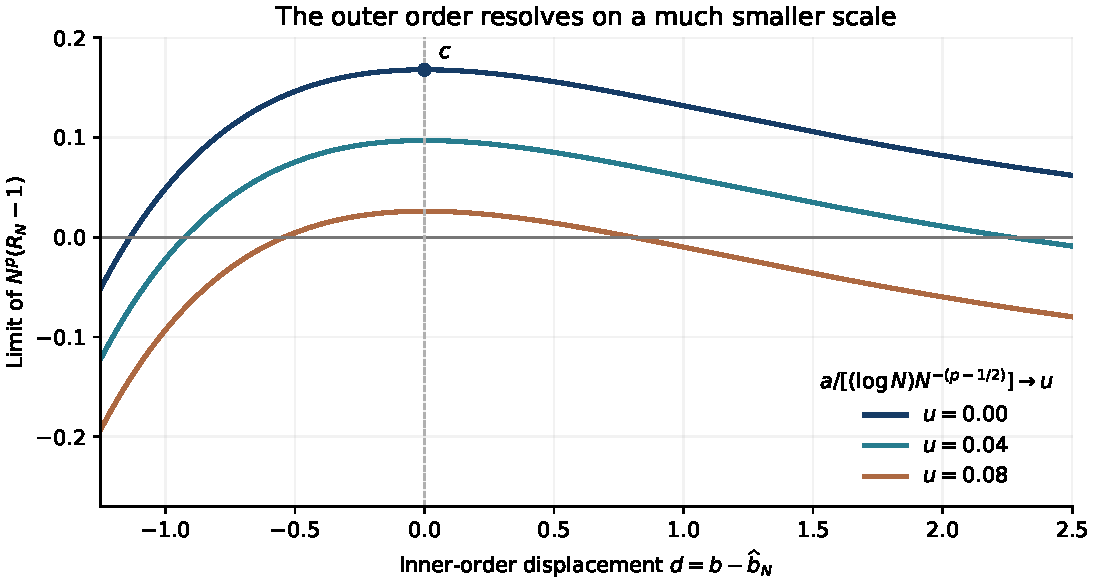
\includegraphics[width=.93\textwidth]{figures/order_plane_profile.pdf}
 \caption{The exact limiting function in
 Proposition~\ref{ord:prop:order-profile}, at three values of the scaled
 outer order $u$. The maximum $c$ occurs at $u=d=0$. These curves depict
 the proved limit; they are not finite-$N$ approximation error claims.}
 \label{ord:fig:profile}
\end{figure}
